\subsubsection{Proton Background}\label{section:star_background_proton}
Secondary particles can be created due to the interaction of particles with detector dead-material.
The proton sample contains background from such protons knocked out  from the~detector materials~\cite{STAR:spectra}. Most of these protons have large $\textrm{DCA}$ and are not reconstructed as primary particles. However, the rest with small $\textrm{DCA}$  are included in the primary track sample. Antiprotons do not have knockout background, hence the flat $\textrm{DCA}$ tail is almost absent from their $\textrm{DCA}$ distributions.

\begin{figure}[h!]
	\centering
	\begin{subfigure}{.49\textwidth}
		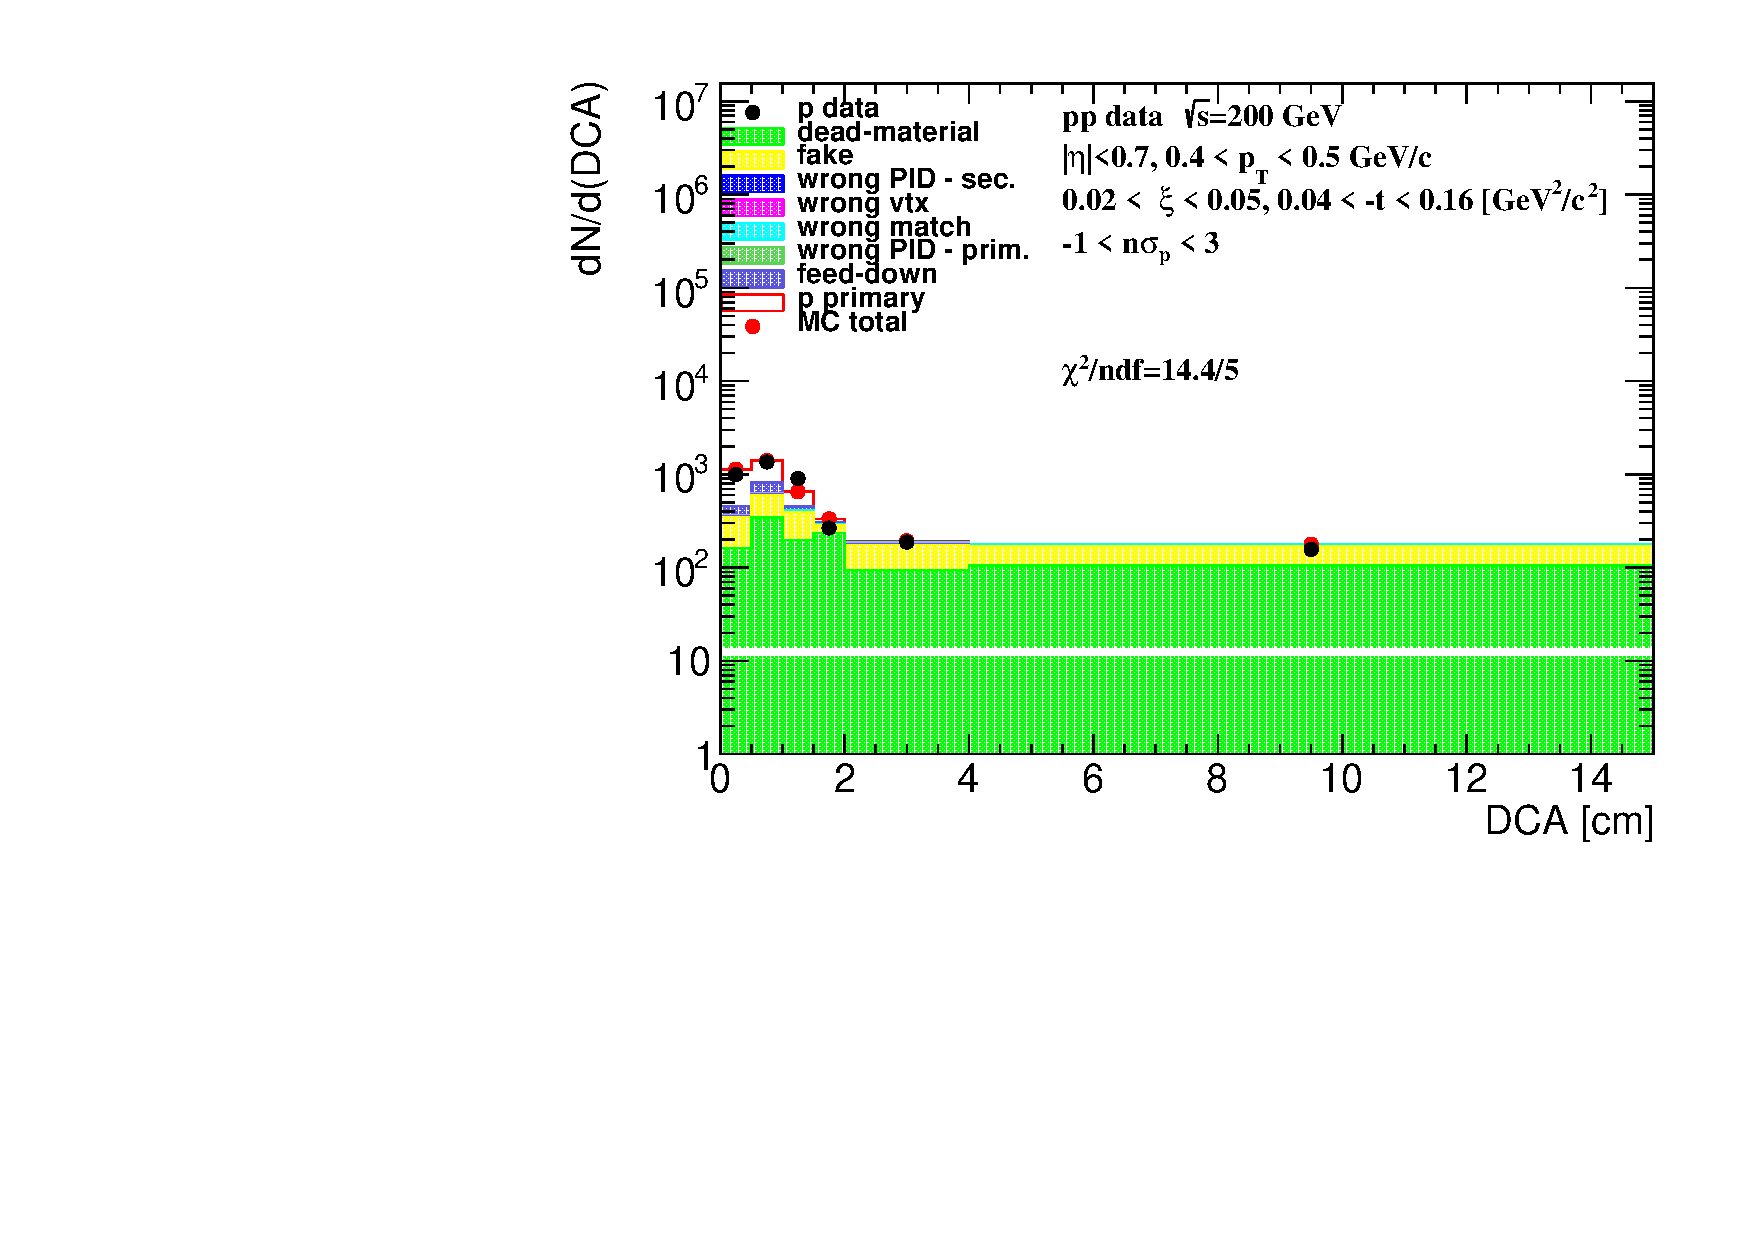
\includegraphics[width=\linewidth, page=1]{chapters/chrgSTAR/img/DCAproton/background_p_0.pdf}
	\end{subfigure}
	\begin{subfigure}{.49\textwidth}
		\includegraphics[width=\linewidth, page=2]{chapters/chrgSTAR/img/DCAproton/background_p_0.pdf}
	\end{subfigure}
	\begin{subfigure}{.49\textwidth}
		\includegraphics[width=\linewidth, page=4]{chapters/chrgSTAR/img/DCAproton/background_p_0.pdf}
	\end{subfigure}
	\begin{subfigure}{.49\textwidth}
		\includegraphics[width=\linewidth, page=5]{chapters/chrgSTAR/img/DCAproton/background_p_0.pdf}
	\end{subfigure}
	\caption{The $\textrm{DCA}$ distributions of protons for $0.4<p_T<0.5$~GeV/c shown for single range of $0.02<\xi<0.05$ (shown in log and linear scale in left and right column, respectively). The MC  constributions are shown after scaling the dead-material template  to data. (top) Background enriched samples were used in the normalization procedure, whereas (bottom) the proton background was estimated from the nominal sample.}
	\label{fig:bkg_proton}
\end{figure}

In order to correct for the knock-out background protons, sample enriched in proton background  was used for background normalization, where $\textrm{DCA}_{xy}$, $\textrm{DCA}_z$ and $d_0$ cuts were abandoned. Additionally, at least one, instead of exactly one,  reconstructed vertex was allowed in this sample.  \Cref{fig:bkg_proton,fig:bkg_proton_bar} show the~$\textrm{DCA}$ distributions of protons and antiprotons, respectively, for  nominal (bottom) and background enriched (top) samples. The distributions for other $p_\textrm{T}$ and $\xi$ regions are shown in Appendix~\ref{appendix:DCA_proton}.
The protons and antiprotons are selected by a $dE/dx$ cut of $-1 < n\sigma_{p,\bar{p}} < 3$ where $n\sigma_{p,\bar{p}}$ is given by Eq.~\eqref{eq:nsigma}. The fraction of knock-out protons within the selected sample is determined via a MC template normalization method. The templates of reconstructed tracks with $dE/dx$ corresponding to the~proton and antiproton are obtained from MC separately for:
\begin{itemize}
	\item primary (anti)protons,
	\item knock-out background protons (labeled as dead-material),
	\item fake tracks,
	\item secondary particles with $dE/dx$ of (anti)proton (labeled as wrong PID - sec.),
	\item tracks associated with primary (anti)protons, but with the reconstructed vertex  not matched to true-level primary vertex (labeled as wrong vtx),
	\item reconstructed track is partially matched to true-level particle (labeled as wrong match, track to true-level particle matching is described in~\ref{section:star_TPCeffi}), i.e.  track and true-level particle have appropriate number of common hit points but the distance between true-level particle and track is too large, $\delta^2\left(\eta,\phi\right)>\left(0.15\right)^2$, 
	\item primary particles with $dE/dx$ of (anti)proton (labeled as wrong PID - prim.),
	\item (anti)proton as a product of short-lived decays, mainly $\Lambda^0$ (labeled as feed-down).
\end{itemize}



First, the background enriched sample was used  (Fig.~\ref{fig:bkg_proton}, top), where the template of knock-out background protons was normalized to the number of events in the fake-subtracted tail of the $\textrm{DCA}$ distribution, $2<\textrm{DCA}<15$~cm. Next the knock-out proton and fake background was subtracted from the $\textrm{DCA}$ distribution and the sum of other templates was normalized to the number of events in the signal region,  $\textrm{DCA}<1.5$~cm. 

\begin{figure}[h!]
	%\vspace{-1cm}
	\centering
	\begin{subfigure}{.49\textwidth}
		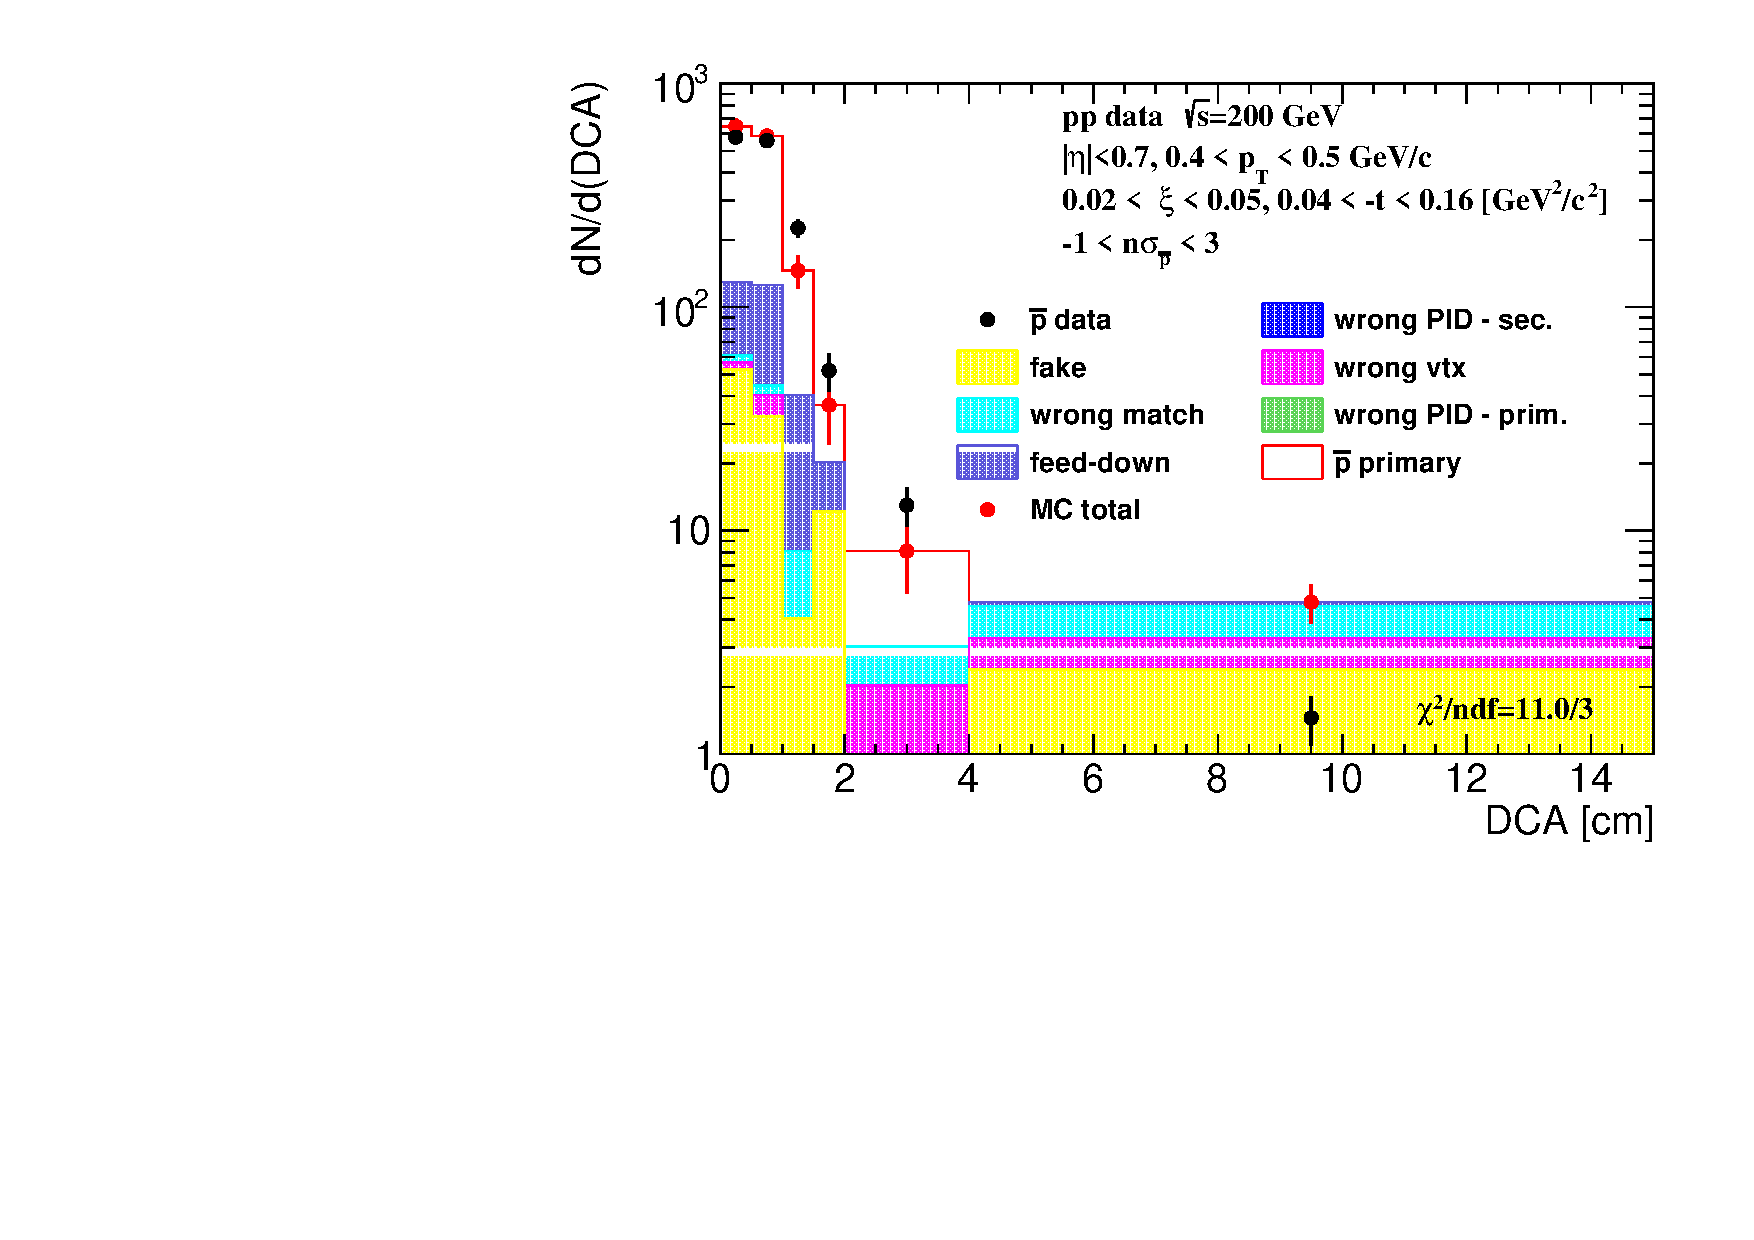
\includegraphics[width=\linewidth, page=1]{chapters/chrgSTAR/img/DCAproton/background_p_bar_0.pdf}
	\end{subfigure}
	\begin{subfigure}{.49\textwidth}
		\includegraphics[width=\linewidth, page=2]{chapters/chrgSTAR/img/DCAproton/background_p_bar_0.pdf}
	\end{subfigure}
	\begin{subfigure}{.49\textwidth}
		\includegraphics[width=\linewidth, page=4]{chapters/chrgSTAR/img/DCAproton/background_p_bar_0.pdf}
	\end{subfigure}
	\begin{subfigure}{.49\textwidth}
		\includegraphics[width=\linewidth, page=5]{chapters/chrgSTAR/img/DCAproton/background_p_bar_0.pdf}
	\end{subfigure}
	\caption{The $\textrm{DCA}$ distributions of antiprotons for $0.4<p_\textrm{T}<0.5$~GeV/c shown for one range of $0.02<\xi<0.05$ (log and linear scale in left and right column, respectively). The MC controbutions are shown as colour histograms. (top) Background enriched and (bottom) nominal samples were used.}
	\label{fig:bkg_proton_bar}
	%\vspace{-1cm}
\end{figure}

The fraction of the knock-out proton background in the signal region, $\textrm{DCA}<1.5$, was estimated from the nominal sample (Fig.~\ref{fig:bkg_proton}, bottom), where $\textrm{DCA}_{xy}$, $\textrm{DCA}_z$ and $d_0$ track cuts were applied and exactly one reconstructed vertex was required. The normalization of each MC contribution was kept the same as that estimated for the background enriched sample. Figure~\ref{fig:bkg_proton_fit} shows the knock-out proton background as a function of $p_\textrm{T}$ in three ranges of $\xi$. The following functional form was found to describe the
background protons well:
\begin{equation}
f_{\textrm{bkg}}^{p}\left(p_\textrm{T}\right) = p_0\exp\left(p_1p_\textrm{T}\right)
\label{eq:protonBkgParametrization}
\end{equation}
where  $p_0$ and $p_1$ are  free parameters obtained from a~fit. 

The obtained fraction of knock-out background protons is approximately $20\%$ at $p_\textrm{T} = 0.45$ GeV/c
 and less than $10\%$ at $p_\textrm{T} = 1.0$~GeV/c. The fraction of knock-out background protons depends on a number of factors, including the amount of detector material, analysis cuts and the $\xi$ of diffractive proton. 
 
 
 
 Figure~\ref{fig:bkg_proton_bar} shows the corresponding $\textrm{DCA}$ distributions with MC templates for antiprotons, where the background form knock-out particles is not present. The MC templates  fairly well describe the $\textrm{DCA}$ distribution for both, protons and antiprotons. Additionally, there is a small $\left(<1\%\right)$ background  contribution, present for both particles, which also was taken into account and subtracted. It originates from reconstructed tracks which have the appropriate number of common hit points with true-level particle, but the distance between them is too large, i.e. $\delta^2\left(\eta,\phi\right)>\left(0.15\right)^2$.
 
 %\captionsetup{format=plain,indention=0pt,justification=justified}
 \begin{figure}[h!]% \begin{wrapfigure}{r}{0.45\textwidth}
 	\centering
 	%\vspace{-20pt}
 	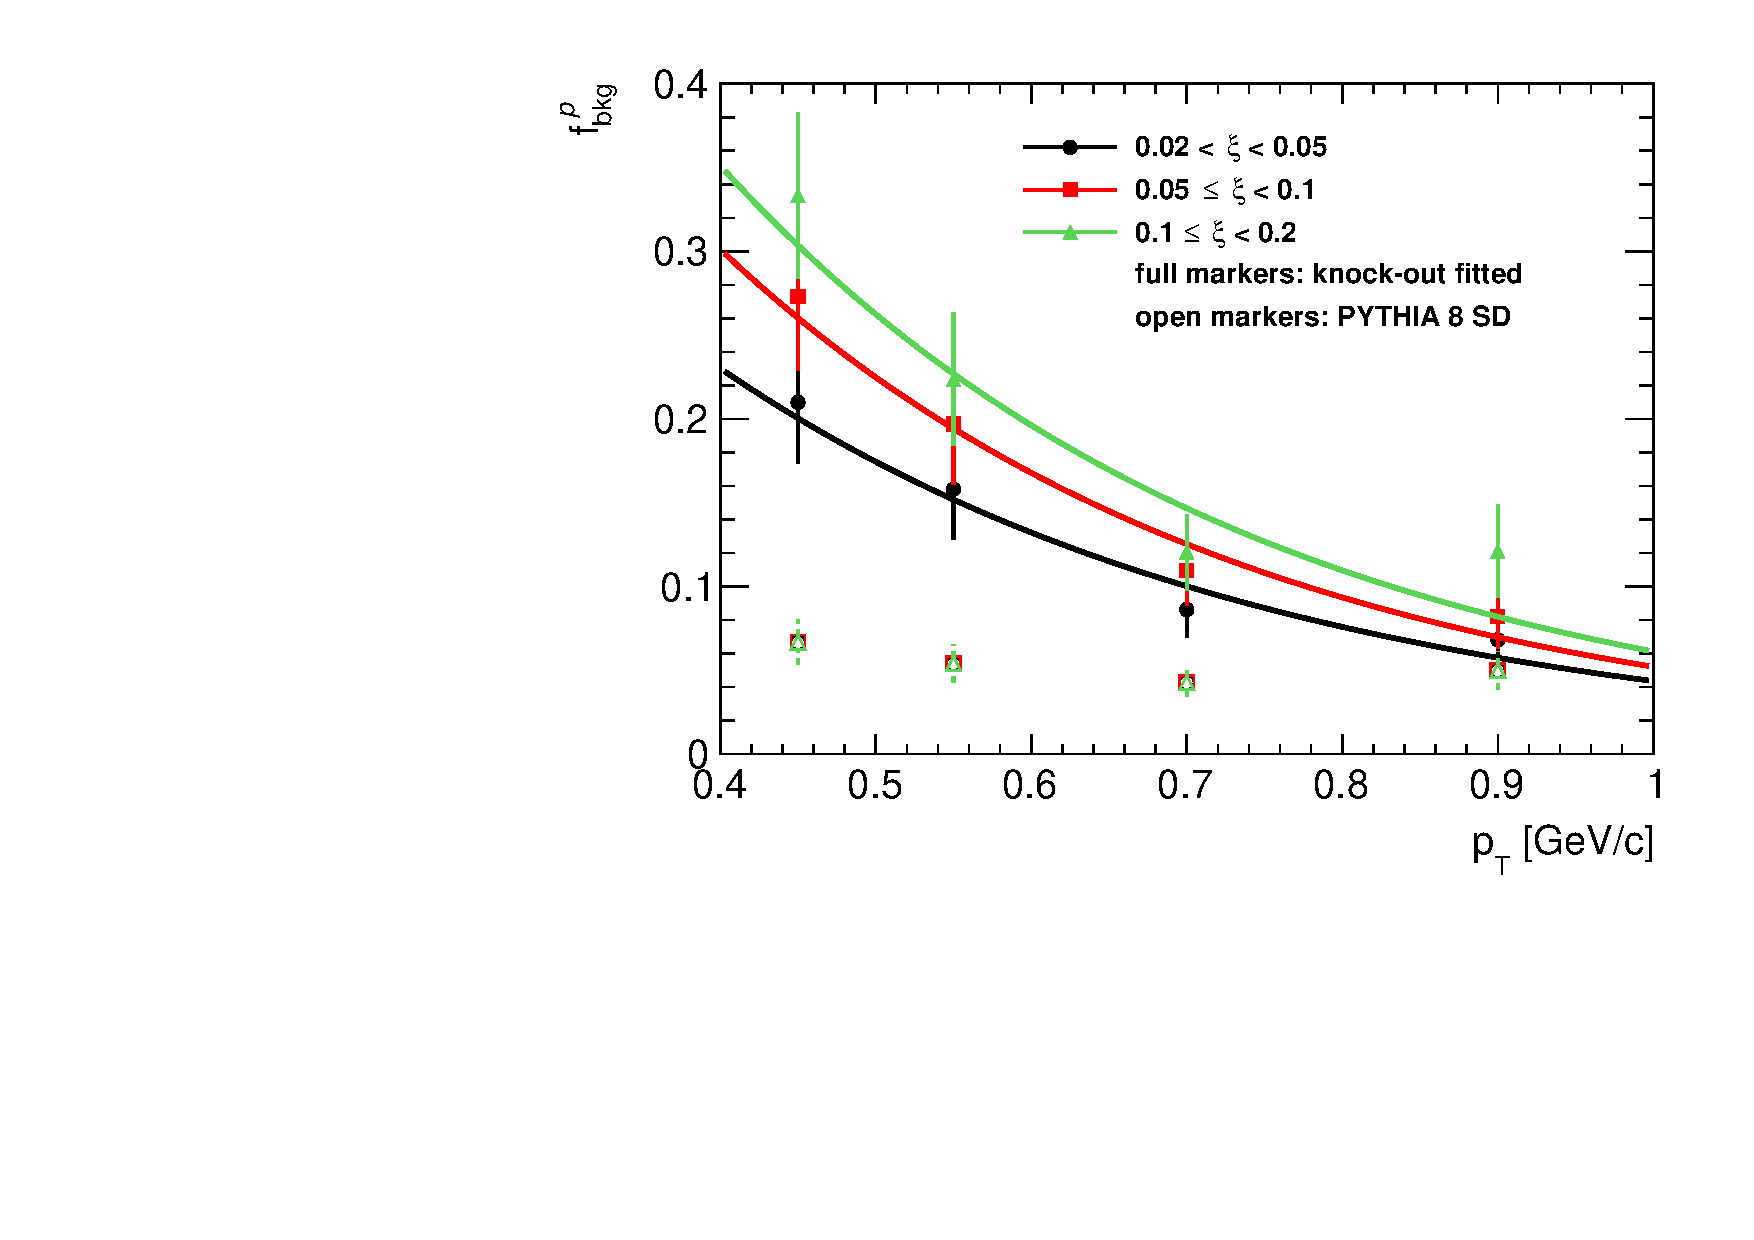
\includegraphics[width=0.8\linewidth, page=1]{chapters/chrgSTAR/img/DCAproton/bkg_p.pdf}
 	%\vspace{-20pt}
 	\caption{The fraction of knock-out proton background  as a function of $p_\textrm{T}$ in three ranges of $\xi$  with  fitted parametrizations.}
 	%\vspace{-80pt}
 	\label{fig:bkg_proton_fit}
 \end{figure}
 %\captionsetup{format=default,indention=0pt,justification=justified}
 %\FloatBarrier
 
 \subsubsection{Systematic Uncertainty Related to Proton Background} 
The method of   knock-out proton background estimation  introduces independent systematic uncertainties which are added in quadrature. 

First, the normalization interval of the  knock-out   proton  background template in the background enriched sample was changed to $4<\textrm{DCA}<15$~cm. This introduced a relative systematic uncertainty of up to $30\%$ for $p_\textrm{T}\approx 1.0$~GeV/c. 

 \begin{figure}[h!]
 	\centering
 	\begin{subfigure}{.49\textwidth}
 		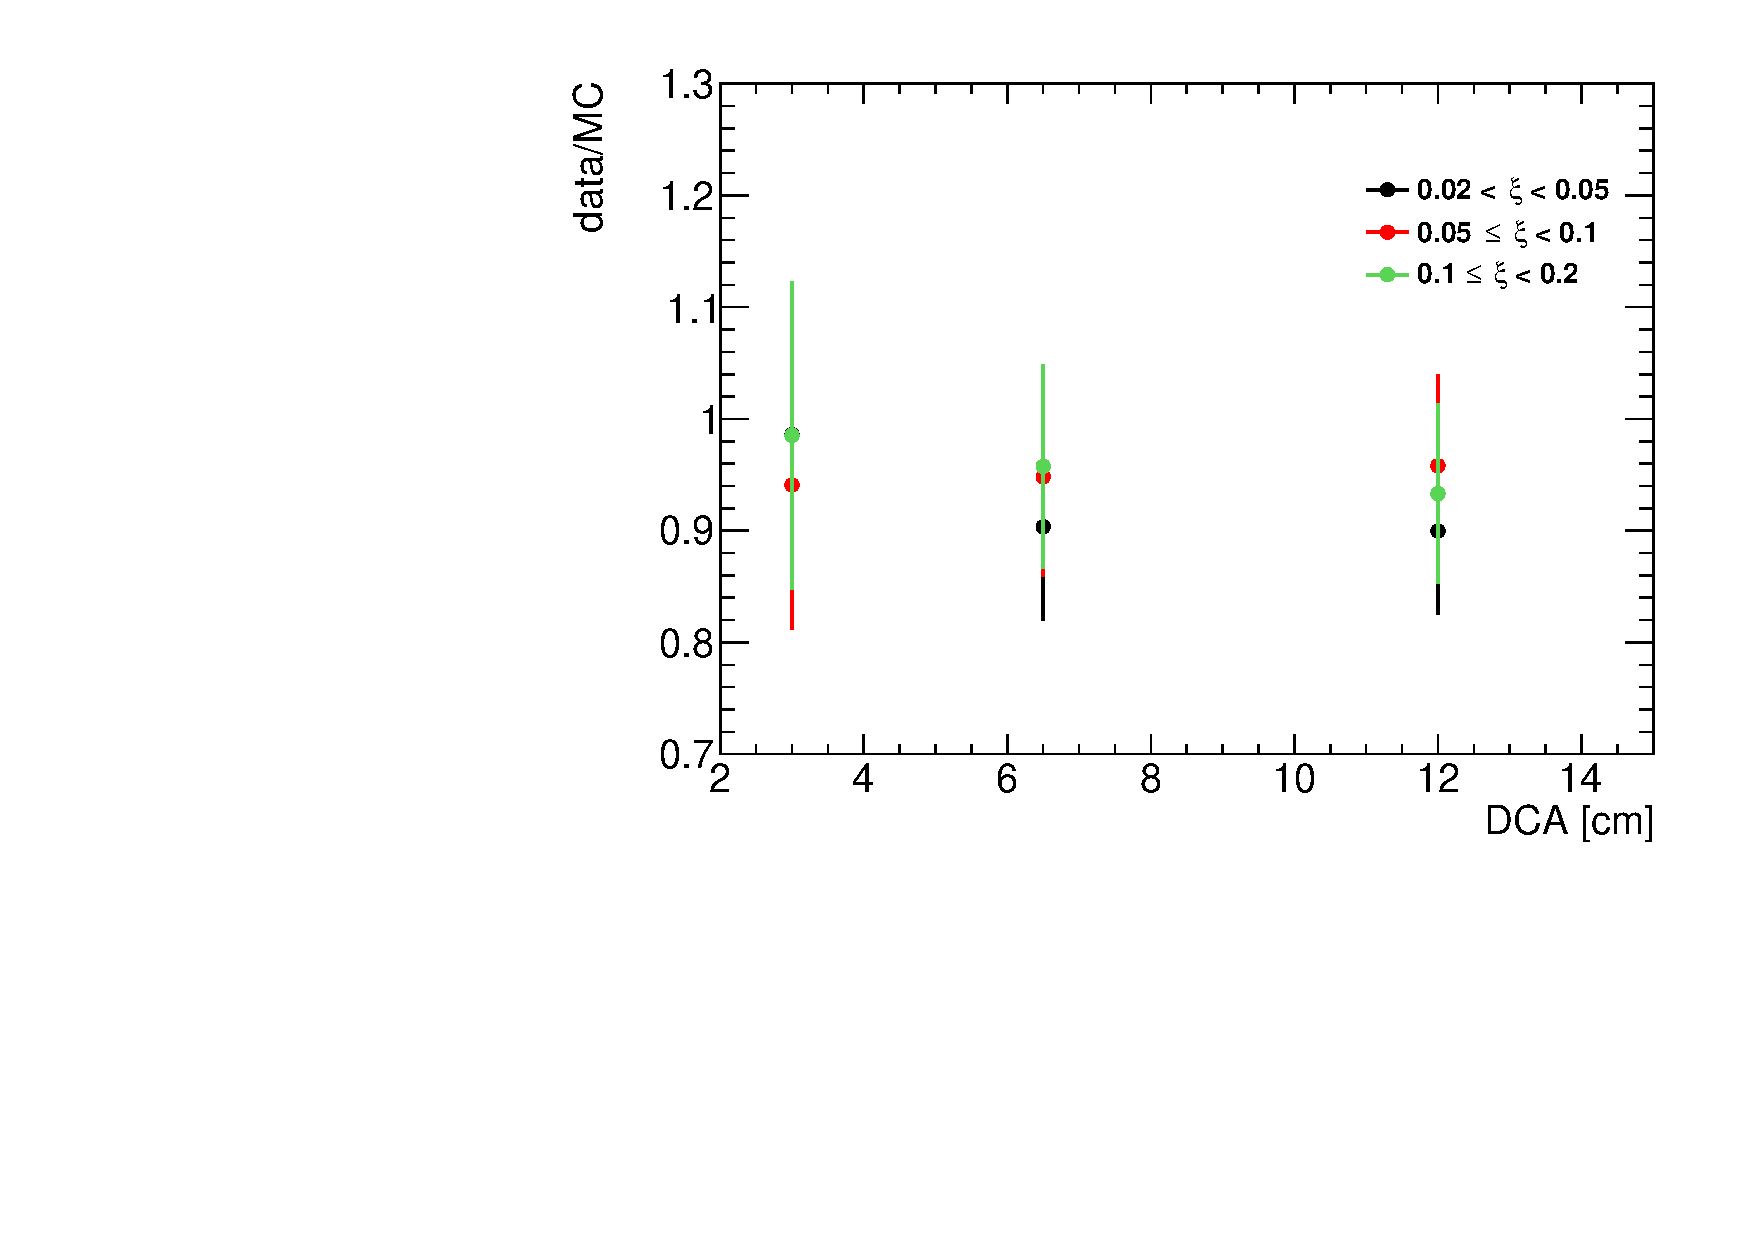
\includegraphics[width=\textwidth,page=1]{chapters/chrgSTAR/img/DCAproton/Ratio.pdf}
 	\end{subfigure}%\label{fig:protonBkgSystRatio}
 	\begin{subfigure}{.49\textwidth}
 		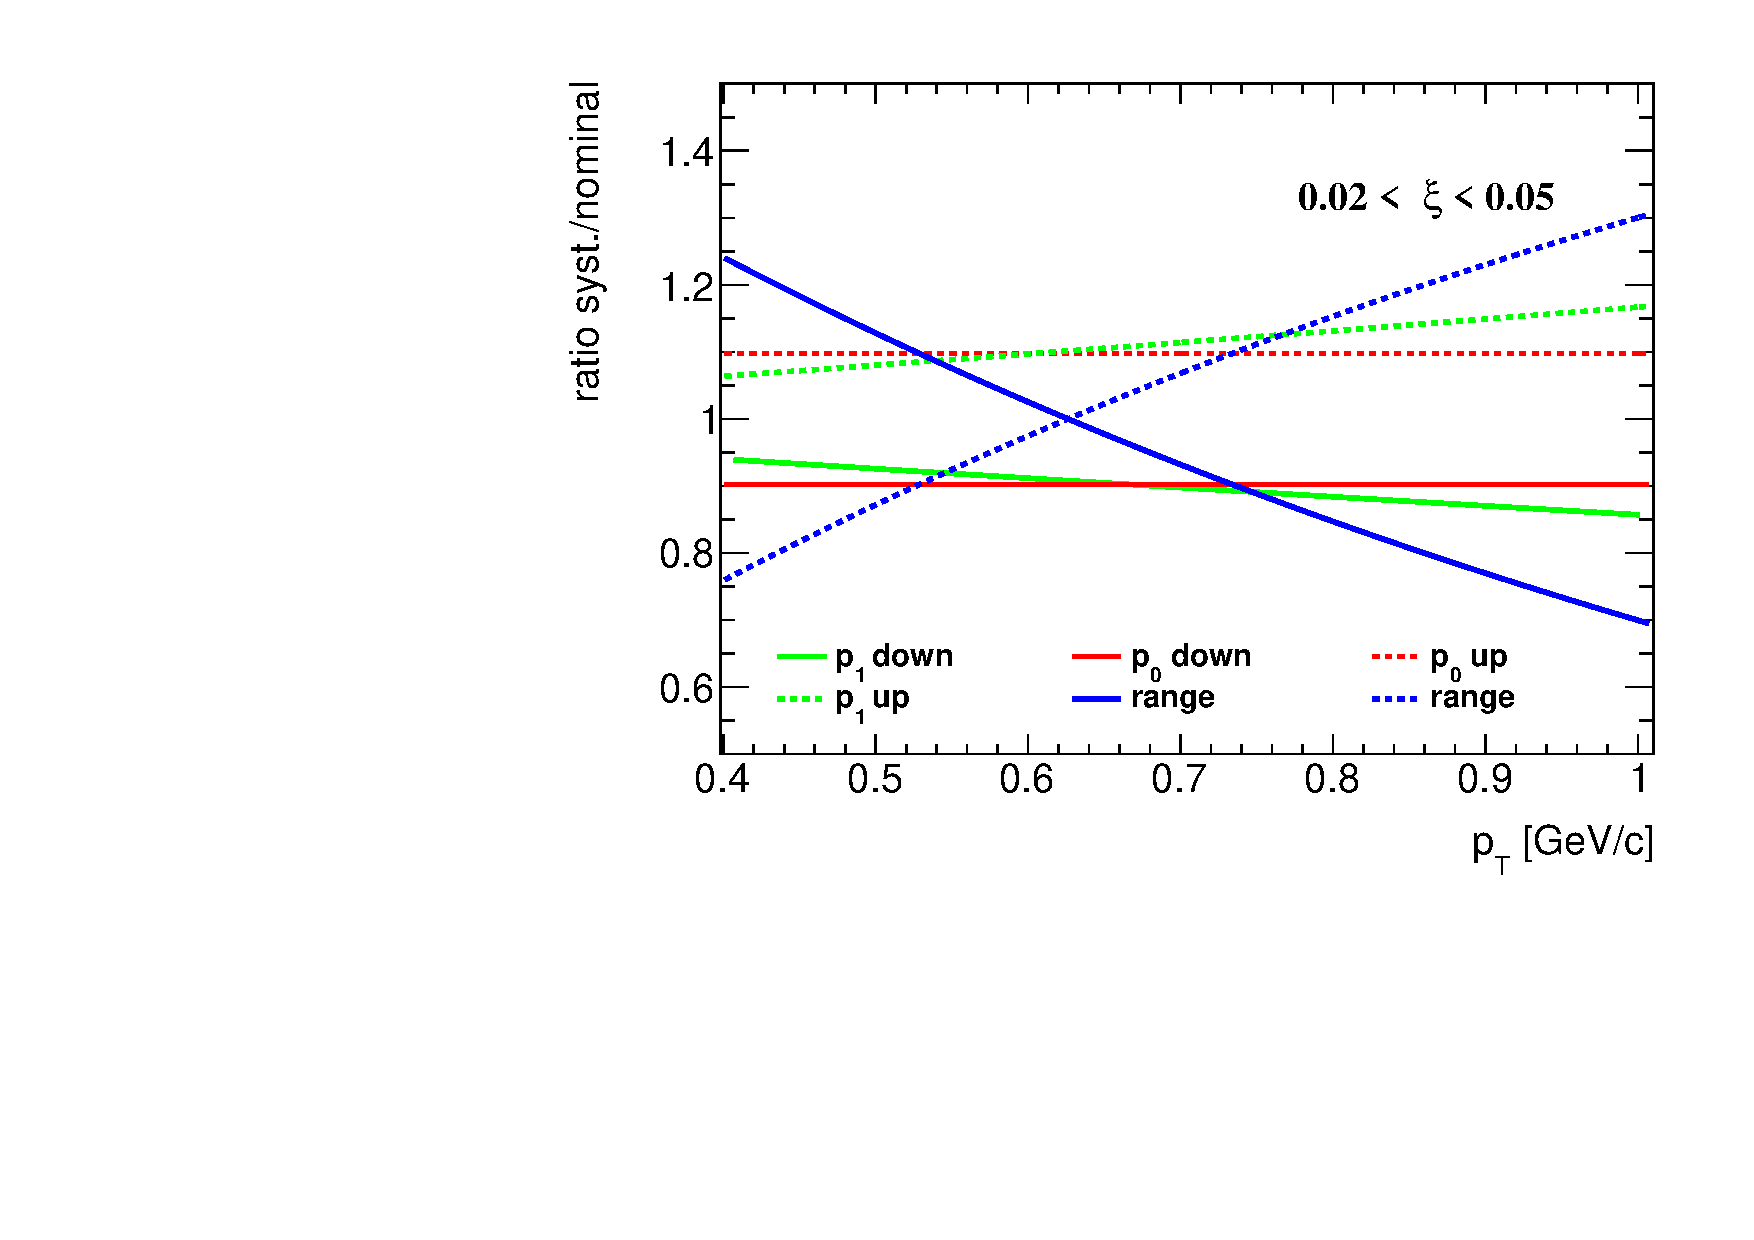
\includegraphics[width=\textwidth,page=1]{chapters/chrgSTAR/img/DCAproton/p_bkg.pdf}
 	\end{subfigure}
 	\begin{subfigure}{.49\textwidth}
 		\includegraphics[width=\textwidth,page=2]{chapters/chrgSTAR/img/DCAproton/p_bkg.pdf}
 	\end{subfigure}
 	\begin{subfigure}{.49\textwidth}
 		\includegraphics[width=\textwidth,page=3]{chapters/chrgSTAR/img/DCAproton/p_bkg.pdf}
 	\end{subfigure}
 	\caption{(top left) Data to MC ratio of  the  number of events in the background dominated region in three ranges of $\xi$ with fitted functional form given by Eq.~\eqref{eq:slopeBkgFit}. (top right and bottom) Components of the systematic uncertainty related to the  knock-out background protons contribution in three $\xi$ ranges. }
 	\label{fig:protonBkgSyst}
 	
 	%\vspace{-2.5cm}
 \end{figure}

The  knock-out proton background contribution was  parameterized as  it is shown in  Eq.~\eqref{eq:protonBkgParametrization}. The systematic uncertainty related to the fit procedure was estimated by varying the   parameters, $p_0$ and $p_1$, by their statistical uncertainties ($\pm1\sigma$).  As a result, a~relative systematic uncertainties of about $10\%$ were obtained.


 
 Figure~\ref{fig:protonBkgSyst} (top left) shows the data to MC ratio of  the  number of events in the background dominated region, $2<\textrm{DCA}<15$~cm. The shape of the $\textrm{DCA}$ distribution in data  differs from that observed in simulation. Thus, the following functional form was used to estimate the slope between data and MC:
\begin{equation}
\frac{\textrm{data}}{\textrm{MC}}\left(\textrm{DCA}\right) = A(\textrm{DCA}-8.5)+B
\label{eq:slopeBkgFit}
\end{equation}
where $A$ (slope) and  $B$ are fit free parameters. An extrapolation of the slope was used to estimate how many
more tail-like tracks would fit into the signal region and a systematic uncertainty, which varies up to $5\%$ for $0.02< \xi<0.05$, was introduced. 




All above components of the systematic uncertainty related to the knock-out proton background are shown in Fig.~\ref{fig:protonBkgSyst}.
 
 
 


 
  %\FloatBarrier